\documentclass[../../dissertation.tex]{subfiles}
\begin{document}
% 	    \subsection{[TEMP Artigos relevantes] }
% 	        MAIS MOEDAS.
% 	        aharonov1993 - Pasta introqw/Coin \\
% 	        \textbf{aharonov2001 - Pasta introqw/Coin} - definiçao da QW  ;shift operator mod n \\
% 	        ambainis2001 - Pasta introqw/Coin \\
% 	        carteret2005- Implementacao - Pasta introqw/Coin \\
% 	        inui2003 -  - Pasta introqw/Coin \\
% 	        kendon2006 - Introducao historia CQ - Pasta introqw/Coin \\
% 	        shenvi2002 - Relacao com grover pg. 10\\
% 	        Resto da pasta.

% 	    \subsection{Texto}




In the quantum case, the walker is a quantum system whose position \textit{x} on the line is described by a vector $\ket{x}$ in Hilbert Space. The next position of the system is determined by a unitary operator, which can be viewed as a quantum coin.
%TODO: \textcolor{red}{O operador unitário não é somente da moeda, precisa falar do espaço do caminhante também}
The analogy is, if the coin is tossed and rolls "heads", for example, the system transitions to position $\ket{x+1}$, otherwise it advances to $\ket{x-1}$. The Hilbert space of the system is $\mathscr{H} = \mathscr{H}_{C} \otimes \mathscr{H}_{P}$, where $\mathscr{H}_{C}$ is the two-dimensional Hilbert space associated with the "coin" and $\mathscr{H}_P$ is the one-dimensional lattice's Hilbert space. One of the most commonly used coins is the Hadamard operator, which is the one chosen for this example.\par
The transition from $\ket{x}$ to either $\ket{x+1}$ or $\ket{x-1}$ must be described by a unitary operator, the \textit{shift operator} 
%TODO: \textcolor{red}{precisa descrever a moeda também e como ela funciona no unitário e acredito que as equações estejam trocadas}
\begin{gather}
	\mathcal{S} \ket{0}\ket{x} = \ket{0}\ket{x-1}\\
	\mathcal{S} \ket{1}\ket{x} = \ket{1}\ket{x+1}
\end{gather}
that can also be described by
\begin{equation}
	S = \ket{0}\bra{0} \otimes \sum_{x=-\infty}^{x=\infty} \ket{x+1}\bra{x} + \ket{1}\bra{1}\otimes \sum_{x=-\infty}^{x=\infty} \ket{x-1}\bra{x}.
\end{equation}
It follows that the operator that describes the dynamics of the quantum walk will be given by 
%TODO: \textcolor{red}{Não necessariamente é o Hadamard, poderia ser uma coin qualquer. Você pode explicar também que a H é a sem viés.}
\begin{equation}
	U = S(H\otimes I). \label{coinedUnmarkedOperator}
\end{equation}\par
Consider a quantum system located at $\ket{x = 0}$ with coin state $\ket{0}$, for $t=0$. It's state will be described by
\begin{equation}
	\ket{\Psi(0)} = \ket{0}\ket{x=0},
	\label{eq:7}
\end{equation}
and after $t$ steps the walker's state will be
\begin{equation}
	\ket{\Psi(t)}=U^{t}\ket{\Psi(0)},
\end{equation}
more explicitly
\begin{equation}
	\ket{\Psi(0)}\xrightarrow[]{\text{$U$}}\ket{\Psi(1)}\xrightarrow[]{\text{$U$}}\ket{\Psi(2)}\xrightarrow[]{\text{$U$}} (...) \xrightarrow[]{\text{$U$}}\ket{\Psi(t)}.
\end{equation}\par
After applying the Hadamard operator followed by the shift operator twice the respective system states are 
%TODO: \textcolor{red}{seria bom especificar que é na moeda, ou até mesmo dizer que o quantum walk consiste da aplicação da moeda e logo em seguida o shift}
\begin{gather}
	\ket{\Psi(1)} = \frac{\ket{0}\ket{x=-1}+\ket{1}\ket{x=1}}{\sqrt{2}}\label{eq:10}\\
	\ket{\Psi(2)} = \frac{\ket{0}\ket{x=-2}+\ket{1}\ket{x=0}+\ket{0}\ket{x=0}-\ket{1}\ket{x=2}}{2}\label{eq:11}\\
\end{gather}
If one were to measure the system after each application of $\mathcal{U}$, it would be expected to see the walker at $x=1$ 50\% of the time and at $x=-1$ for the remainder, after the first iteration (\ref{eq:10}). Measure the system $t$ times and the result is a binomial probability distribution. The conclusion is that repetitive measurement of a coined quantum walk system reduces to the classical case, which means that any desired quantum behaviour is lost. \par
It is possible, however, to make use of the quantum correlations between different positions to generate constructive or destructive  interference, by applying the Hadamard and shift operators successively without intermediary measurements.
The consequences of interference between states are very apparent in
\begin{equation}
	\ket{\Psi(3)} = \frac{\ket{1}\ket{x=-3}-\ket{0}\ket{x=-1}+2(\ket{0}+\ket{1})\ket{x=1}+\ket{0}\ket{x=3}}{2\sqrt{2}}\label{eq:12}.
\end{equation}
Even though an unbiased coin was used, this state is not symmetric to the origin and the probability distributions will not be centered in the origin. Moreover, the standard deviation will not be $\sqrt{t}$.\par
%TODO: \textcolor{red}{Bom, faltou dizer qual o desvio padrão da quantum walk que é $t$ e esse $\sqrt{t}$ é da clássica. Precisa justificar com alguma referência também}\par
The quantum walk is said to be \textit{ballistic} since its standard deviation is proportional to $t$ \cite{andraca2012} meaning exponentially faster hitting times in certain graphs \cite{childs2002,fahri98} which can be advantageous in problems that involve visiting certain vertices in a graph. There are also studies that show that a quantum walk may have advantages in element distinctness \cite{ambainis2003} and spatial search \cite{childs2004} problems. 
%TODO: \textcolor{red}{talvez esse parágrafo deva subir, porque você fala de desvio padrão muito antes}

In order to study this distribution, a simulation of the coined quantum walk was coded in \textit{Python}. Using the Hadamard coin and the aforementioned initial condition, the resulting probability distribution is:

\begin{figure}[!h]
	\centering
	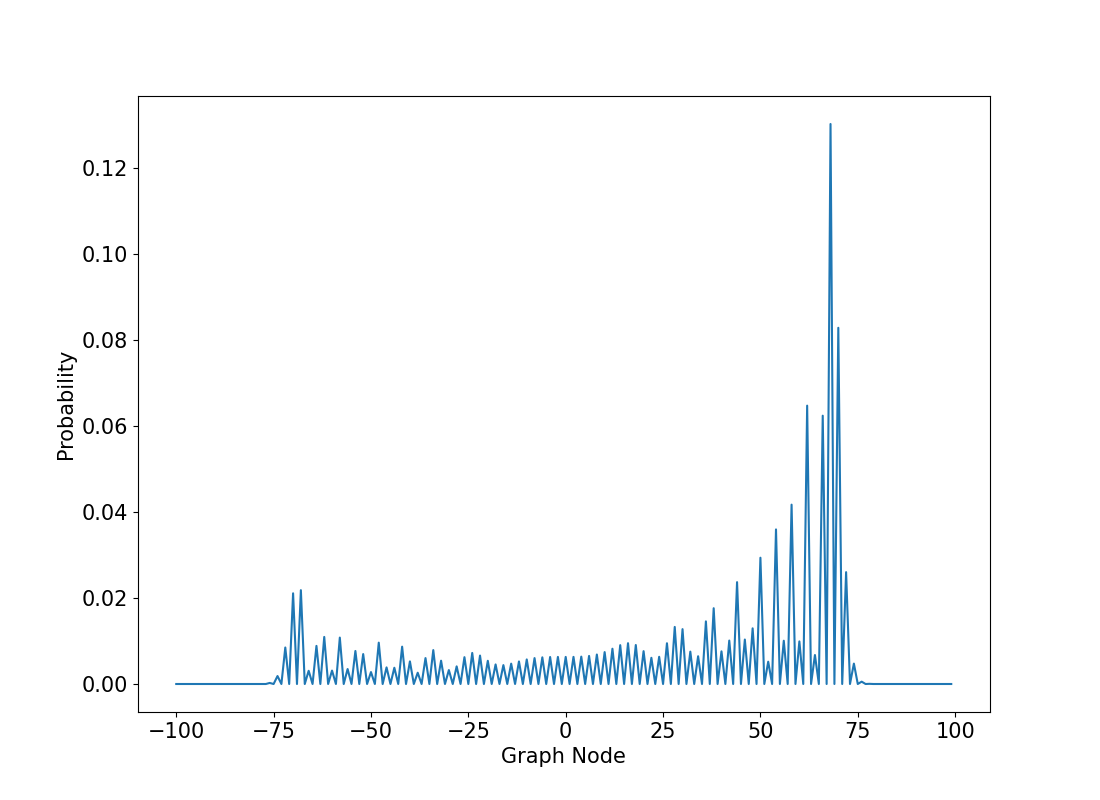
\includegraphics[scale=0.40]{img/CoinedQuantumWalk/Coinedpsi00.png}
	\caption{Probability distribution for the coined quantum walk on a line, after 100 steps, with initial condition $\ket{\Psi(0)}=\ket{0}\ket{x=0}$ and the Hadamard coin.} 
	\label{fig:fig1}
\end{figure}

Analyzing the plot, it is noticeable that the distribution is asymmetric, the probability amplitude of finding the walker at the right-hand side is much larger than at the left, with a peak around $x=\frac{100}{\sqrt{2}}$. Regardless of number of steps, this peak is always present (albeit in varying positions), which is to say that the walker can always be found moving in a uniform fashion away from the origin, further confirming the quantum walk's ballistic behaviour.\par 
%TODO: \textcolor{red}{agora penso que um grafo sobre desvio padrão seria bom para ilustrar, porque o desvio padrão foi muito comentado ao longo do texto}\par
Another interesting case study is to find if this behaviour is preserved for a symmetric distribution around the origin. For this purpose, one must first understand where the asymmetry comes from. The Hadamard operator flips the sign of state $\ket{1}$, hence more terms are cancelled when the coin state is $\ket{1}$. Since $\ket{0}$ was defined to induce movement to the right, the result is as shown in \ref{fig:fig1}. It then follows that the initial condition 
%TODO: \textcolor{red}{cuidado com a notação embaixo dos kets, e esse sinal negativo é necessário? acredito que não.}
\begin{equation}
	\ket{\Psi(0)} = -\ket{1}\ket{x=0}
	\label{eq:12}
\end{equation}

Will return a mirror image of \ref{fig:fig1}:
\begin{figure}[!h]
	\centering
	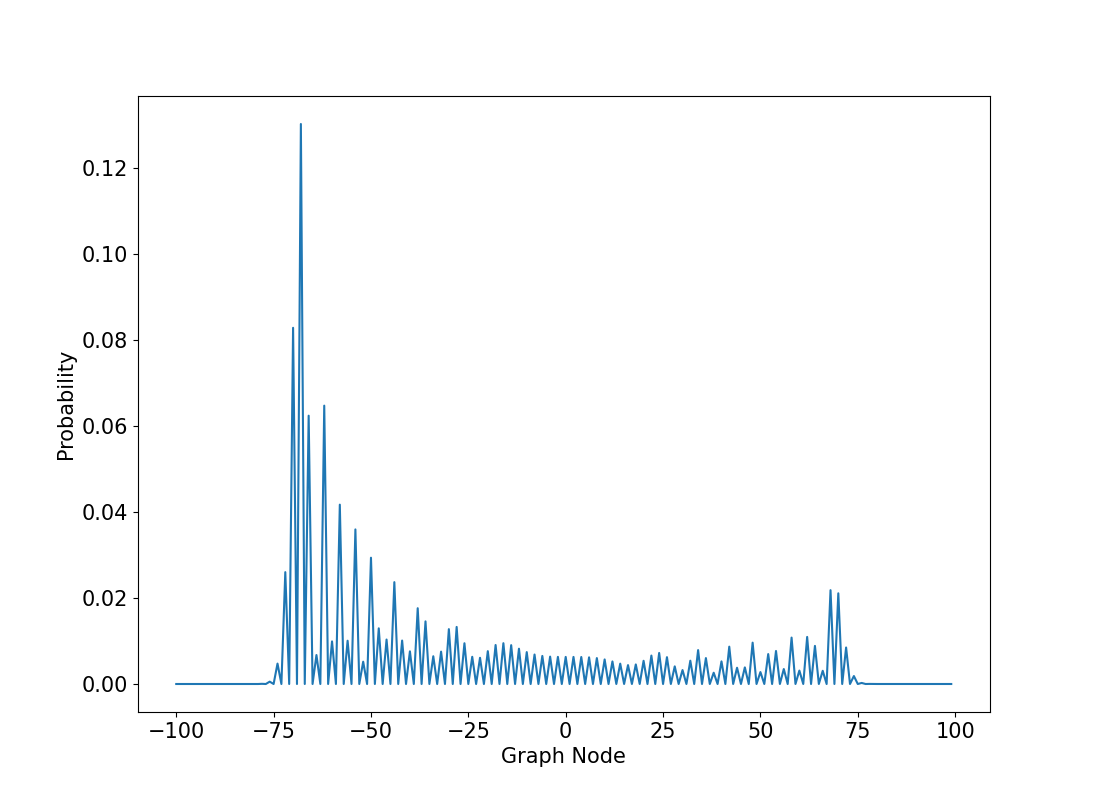
\includegraphics[scale=0.40]{img/CoinedQuantumWalk/Coinedpsi01.png}
	\caption{Probability distribution for the coined quantum walk on a line, after 100 steps, with initial condition $\ket{\Psi(0)}=-\ket{1}\ket{x=0}$ and the Hadamard coin.} 
	\label{fig:fig2}
\end{figure}

In order to obtain a symmetrical distribution, one must superpose \ref{eq:7} and \ref{eq:12} carefully, as to not cancel terms before the calculation of the probability distribution, by multiplying \ref{eq:12} by the imaginary unit. This works because the entries of the Hadamard operator are real numbers; terms with the imaginary unit will not cancel out with terms without it, thus the walk can proceed to both left and right. The initial condition is then: 
%TODO:\textcolor{red}{o sinal pode ser justificado apenas aqui}
\begin{equation}
	\ket{\Psi(0)} = \frac{\ket{0}-i\ket{1}}{\sqrt{2}}\ket{x=0}
	\label{eq:12}
\end{equation}
With a correspoding plot:
\begin{figure}[!ht]
	\centering
	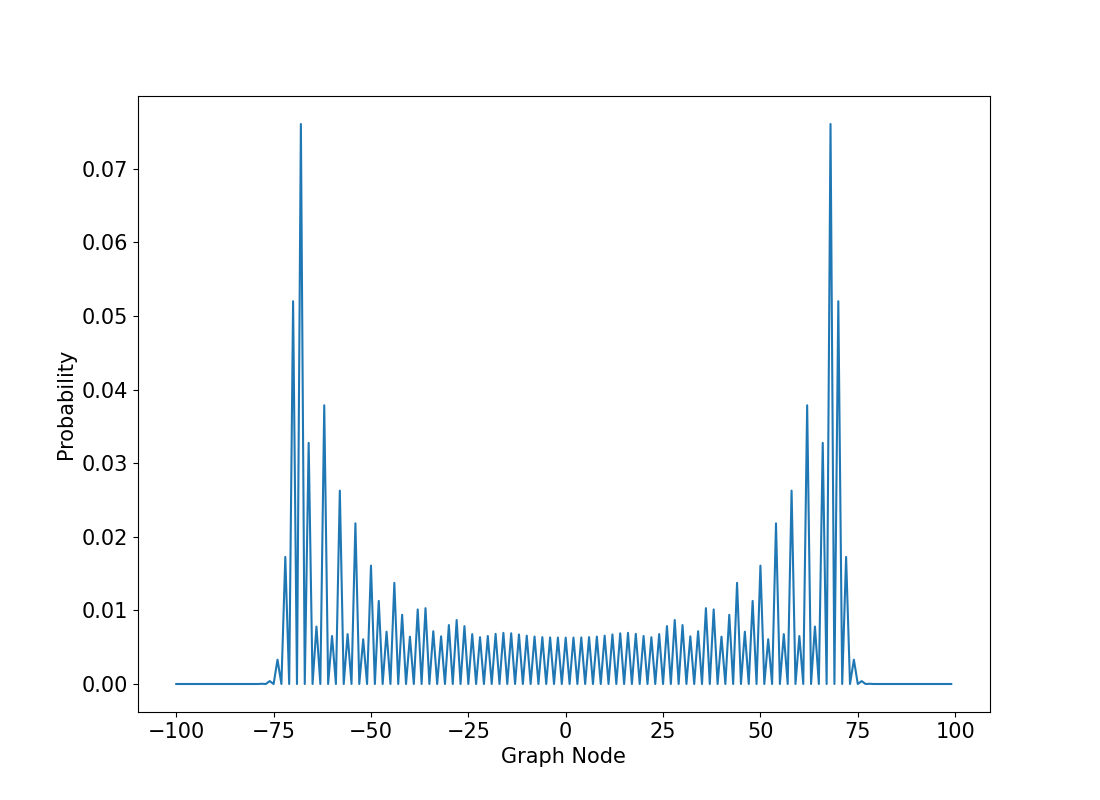
\includegraphics[scale=0.40]{img/CoinedQuantumWalk/Coinedpsi001.png}
	\caption{Probability distribution for the coined quantum walk on a line, after 100 steps, with initial condition $\ket{\Psi(0)}=\frac{\ket{0}-i\ket{1}}{\sqrt{2}}\ket{x=0}$ and the Hadamard coin.} 
	\label{fig:coinedwalk3}
\end{figure}

%TODO: \textcolor{red}{precisa de um fechamento para esta parte, algo que sumarize os resultados, o que veremos nas próximas partes, etc}

\begin{figure}[!h]
	\centering
	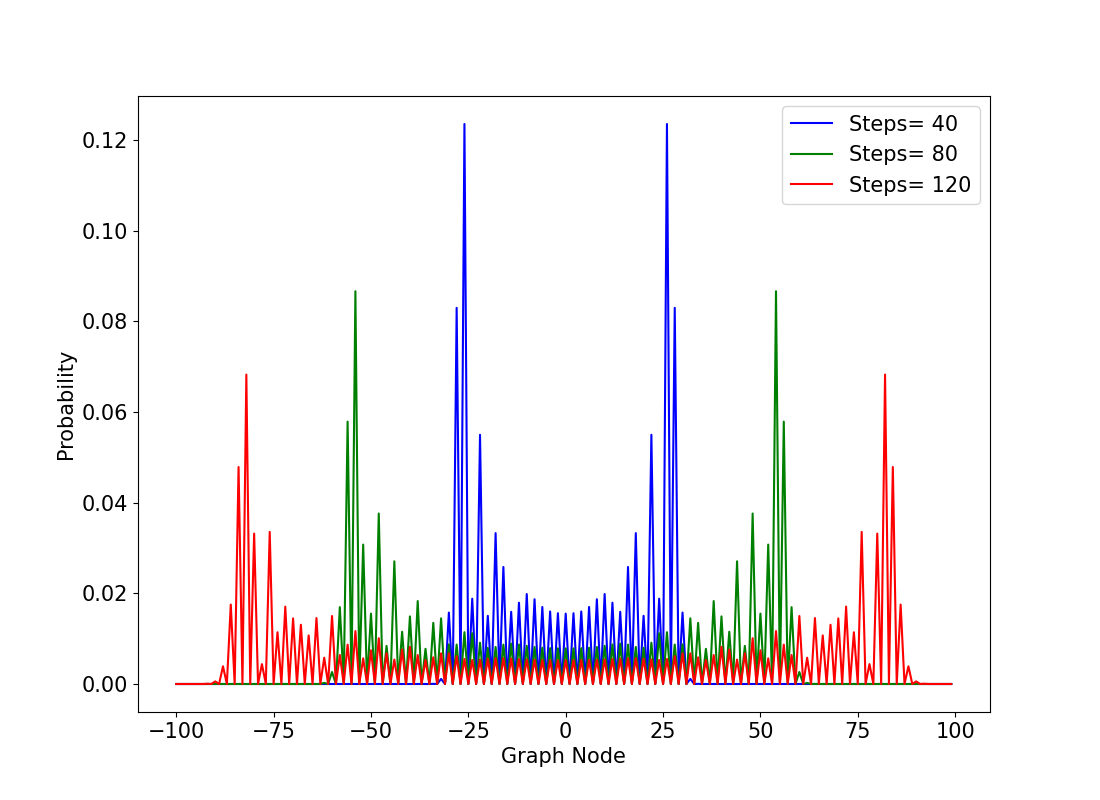
\includegraphics[scale=0.40]{img/CoinedQuantumWalk/CoinedMultiplepsi001.png}
	\caption{Multiple walks temp} 
	\label{fig:coinedwalk3}
\end{figure}

\end{document}
